%% 06_model2_bank_stress.tex
%% Section 6: Model 2 -- Banking Sector Stress Test

\section{Model 2: Banking Sector Stress Test}
\label{sec:model2}

The second model traces how coal stranding propagates to the banking sector through credit exposures. We construct a bipartite bank-coal exposure network from granular loan data, classify coal companies by default status under each scenario, and estimate the resulting credit losses and capital adequacy impacts for each bank.

\subsection{Bank-Coal Exposure Network}
\label{subsec:bipartite_network}

The foundation of our stress test is a bipartite network linking banks to coal companies through identified credit relationships. We construct this network from annual report disclosures of 38 listed banks, which report their largest borrower exposures by company name, loan amount, currency, and sector classification. For coal companies, we identify direct credit facilities, including term loans, revolving credit, project finance, and trade finance, extended by each bank to each coal company in our sample.

Let $W_{b,c}$ denote the exposure of bank $b$ to coal company $c$, measured in USD millions after currency conversion. The exposure matrix $\mathbf{W}$ has dimensions $B \times C$, where $B = 13$ banks with identified coal exposures (of the 38 in our sample) and $C = 27$ coal companies receiving bank credit. The total identified exposure is \$6.1 billion, of which \$3.3 billion (53.8\%) is attributed to specific bank-company pairs. The remaining \$2.8 billion is classified under aggregate categories (foreign banks, syndicated loans, and other domestic banks) that cannot be traced to individual institutions in our sample.

Figure~\ref{fig:network} visualises the bipartite network. The network exhibits substantial concentration: four domestic systemically important banks (D-SIBs), namely Bank Mandiri (BMRI), Bank Negara Indonesia (BBNI), Bank Central Asia (BBCA), and Bank Rakyat Indonesia (BBRI), account for 79\% of identified bank-level coal exposure. BMRI alone holds \$1.2 billion in direct coal lending, representing the largest single-bank exposure in the network. On the coal company side, the top five borrowers absorb over 60\% of total bank credit to the sector.

\begin{figure}[htbp]
\centering
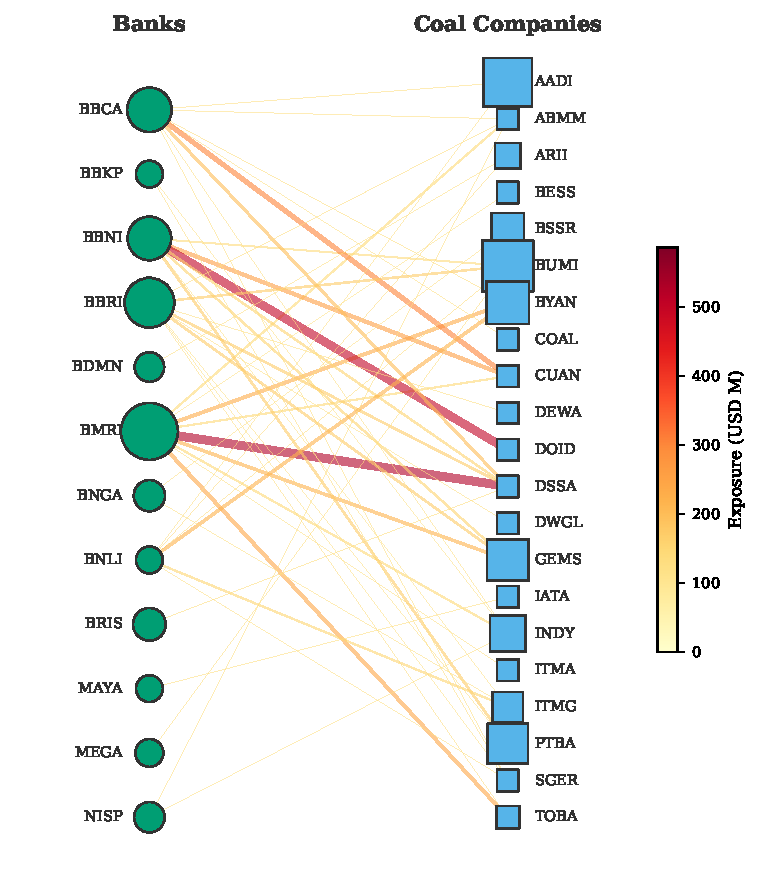
\includegraphics[width=\textwidth]{figures/fig_05.pdf}
\caption{Bipartite bank-coal exposure network. Left nodes represent banks (circle size proportional to total assets); right nodes represent coal companies (square size proportional to annual production). Edge width is proportional to loan exposure in USD millions. The four D-SIBs are highlighted in darker shading.}
\label{fig:network}
\end{figure}

In addition to direct identified exposures, banks hold mining sector loans that may include coal-related lending not individually identified in the bipartite network. We capture these ``indirect'' exposures using the mining loan data from bank financial statements. For bank $b$, the indirect coal exposure is estimated as:
\begin{equation}
\label{eq:indirect}
E_b^{indirect} = M_b - \sum_{c} W_{b,c}
\end{equation}
where $M_b$ is the bank's total mining sector loans (from sectoral loan disclosures) and $\sum_c W_{b,c}$ is its total identified coal exposure. This residual captures lending to unlisted coal companies, coal service providers, and other mining sub-sectors that may be indirectly affected by coal stranding.

\subsection{Credit Loss Model}
\label{subsec:credit_loss}

We model credit losses in two stages: first, we classify each coal company's credit status under each scenario using Model 1 outputs; second, we compute the expected loss for each bank-coal pair.

\subsubsection{Coal Company Default Classification}

Each coal company $c$ is assigned a credit status $S_c^s \in \{\text{Default}, \text{Distressed}, \text{Performing}\}$ under scenario $s$ based on its NPV and equity position:

\begin{equation}
\label{eq:default}
S_c^s = \begin{cases}
\text{Default} & \text{if } NPV_c^s < 0 \\
\text{Distressed} & \text{if } NPV_c^s \geq 0 \text{ and } SV_c^s > 0.50 \cdot E_c \\
\text{Performing} & \text{otherwise}
\end{cases}
\end{equation}
where $E_c$ is the firm's total equity. The rationale is as follows: a negative NPV indicates that the firm's coal operations are value-destroying, implying eventual inability to service debt (default); a positive NPV but stranded value exceeding 50\% of equity indicates material financial stress that elevates credit risk without immediate default; otherwise, the firm remains performing.

Under the BAU scenario, 2 firms default, none are distressed, and 13 are performing; the remaining 20 lack the verified production data needed for NPV-based classification and are assigned a ``no data'' status. Under the 2\textdegree C scenario, 3 firms default and 12 are distressed, with no firms remaining in performing status among those with NPV data. Under the 1.5\textdegree C scenario, 5 firms default and 10 are distressed. This deterioration reflects the severity of the climate-adjusted price paths, which push most producers below breakeven. The 20 firms without NPV data are excluded from the default classification, which means our credit loss estimates are conservative, capturing only losses from the 15 firms with verified cost and production data.

\subsubsection{Loss Given Default}

The loss given default (LGD) varies by credit status:

\begin{equation}
\label{eq:lgd}
LGD_c^s = \begin{cases}
\min\left(1, \frac{|NPV_c^s|}{D_c}\right) & \text{if } S_c^s = \text{Default} \\[6pt]
0.30 \times \frac{SV_c^s}{A_c} & \text{if } S_c^s = \text{Distressed} \\[6pt]
0 & \text{if } S_c^s = \text{Performing}
\end{cases}
\end{equation}
where $D_c$ is total debt and $A_c$ is total assets. For defaulting firms, the LGD is bounded by the ratio of the NPV shortfall to total debt, capped at 100\%. For distressed firms, we apply a conservative 30\% recovery haircut scaled by the stranded value relative to assets, reflecting elevated credit risk without full default. Performing firms incur no losses under our baseline specification, though we relax this assumption in robustness checks (Section~\ref{sec:discussion}).

\subsubsection{Bank-Level Credit Losses}

The total credit loss for bank $b$ under scenario $s$ comprises direct losses from identified exposures and indirect losses from residual mining portfolios:

\begin{equation}
\label{eq:bank_loss}
L_b^s = \underbrace{\sum_{c} W_{b,c} \cdot LGD_c^s}_{\text{Direct losses}} + \underbrace{E_b^{indirect} \cdot \Delta NPL^s \cdot LGD^{generic}}_{\text{Indirect losses}}
\end{equation}

The indirect loss term applies a scenario-dependent NPL increment $\Delta NPL^s$ (calibrated at 0.5\% for BAU, 5\% for 2\textdegree C, and 15\% for 1.5\textdegree C based on the share of stranded firms in the sector) multiplied by a generic LGD of 45\%, consistent with Basel regulatory parameters for corporate exposures in emerging markets.

\subsection{Capital Adequacy Impact}
\label{subsec:capital_adequacy}

We assess the impact on each bank's capital adequacy ratio (CAR) by deducting credit losses from equity capital:

\begin{equation}
\label{eq:car_impact}
CAR_b^{post} = \frac{E_b - L_b^s}{RWA_b}
\end{equation}
where $E_b$ is pre-stress equity capital, $L_b^s$ is the total credit loss, and $RWA_b$ is risk-weighted assets. We hold RWA constant under the assumption that asset migration effects are captured in the LGD specification. The CAR impact in percentage points is:
\begin{equation}
\label{eq:car_delta}
\Delta CAR_b^s = \frac{L_b^s}{RWA_b} \times 100
\end{equation}

We benchmark post-stress CARs against two regulatory thresholds: the OJK minimum CAR of 8\% (applicable to all banks) and the enhanced capital buffer for D-SIBs, which ranges from 10.5\% to 13\% depending on the bank's systemic importance classification.

We further compute the profit impact as the ratio of total credit losses to pre-stress net income, providing a measure of how many years of earnings would be required to absorb the stress losses:
\begin{equation}
\label{eq:profit_impact}
PI_b^s = \frac{L_b^s}{NI_b} \times 100\%
\end{equation}

\subsection{Results}
\label{subsec:model2_results}

Table~\ref{tab:stress_test} presents the stress test results for the 15 most affected banks, while Figure~\ref{fig:car_impact} visualises the post-stress CAR distribution under the 1.5\textdegree C scenario.

\begin{table}[htbp]
\centering
\caption{Bank Stress Test Results: Top 15 Most Affected Banks}
\label{tab:stress_test}
\footnotesize
\setlength{\tabcolsep}{3.5pt}
\begin{tabular}{lrrrrrrrr}
\toprule
Bank & Exposure & Direct & Indirect & Total & CAR & CAR & CAR & Profit \\
 & (\$M) & Loss & Loss & Loss & Before & After & After & Impact \\
 & & (\$M) & (\$M) & (\$M) & (\%) & 2\textdegree{}C (\%) & 1.5\textdegree{}C (\%) & 1.5\textdegree{}C (\%) \\
\midrule
  BMRI & 1,208.6 & 1,055.3 & 589.9 & 1,645.3 & 20.1\% & 19.6\% & 19.2\% & 42.4\% \\
  BNLI & 261.8 & 451.2 & 0.0 & 451.2 & -- & -- & -- & -- \\
  BBRI & 287.6 & 393.7 & 0.0 & 393.7 & 26.6\% & 26.4\% & 26.3\% & 10.3\% \\
  BBNI & 974.9 & 360.0 & 0.0 & 360.0 & 21.1\% & 20.8\% & 20.7\% & -- \\
  BBCA & 441.0 & 61.0 & 84.0 & 145.0 & 28.9\% & 28.8\% & 28.7\% & 4.2\% \\
  MEGA & 21.7 & 29.1 & 36.6 & 65.6 & 25.6\% & 25.1\% & 24.6\% & -- \\
  BNGA & 10.1 & 21.7 & 30.8 & 52.6 & 23.3\% & 23.2\% & 23.1\% & 12.0\% \\
  BDMN & 8.5 & 11.6 & 0.0 & 11.6 & 26.2\% & 26.2\% & 26.1\% & 5.5\% \\
  BBKP & 14.3 & 0.6 & 10.4 & 11.0 & 16.4\% & 16.3\% & 16.2\% & -- \\
  BRIS & 24.1 & 0.0 & 8.2 & 8.2 & 21.5\% & 21.5\% & 21.5\% & -- \\
  PNBN & 0.3 & 0.0 & 2.1 & 2.1 & 34.5\% & 34.5\% & 34.5\% & 1.2\% \\
  NISP & 10.9 & 0.5 & 0.0 & 0.5 & 23.6\% & 23.6\% & 23.6\% & -- \\
  MAYA & 12.4 & 0.0 & 0.0 & 0.0 & -- & -- & -- & -- \\
\midrule
  \textbf{System total} & \textbf{3,276.1} & \textbf{2,384.8} & \textbf{762.1} & \textbf{3,146.8} & & & & \\
\bottomrule
\end{tabular}

\smallskip
\noindent \textit{Notes:} Direct loss = expected loss on coal-sector loans (LGD $\times$ EAD). Indirect loss = second-round contagion via interbank and supply-chain channels. CAR = capital adequacy ratio. Profit impact = total loss as percentage of net income. $^{*}$Bank breaches OJK minimum CAR of 8\%. $^{\dagger}$Bank breaches D-SIB buffer of 10.5\%. System total covers all 13 banks in the sample.
\end{table}


\begin{figure}[htbp]
\centering
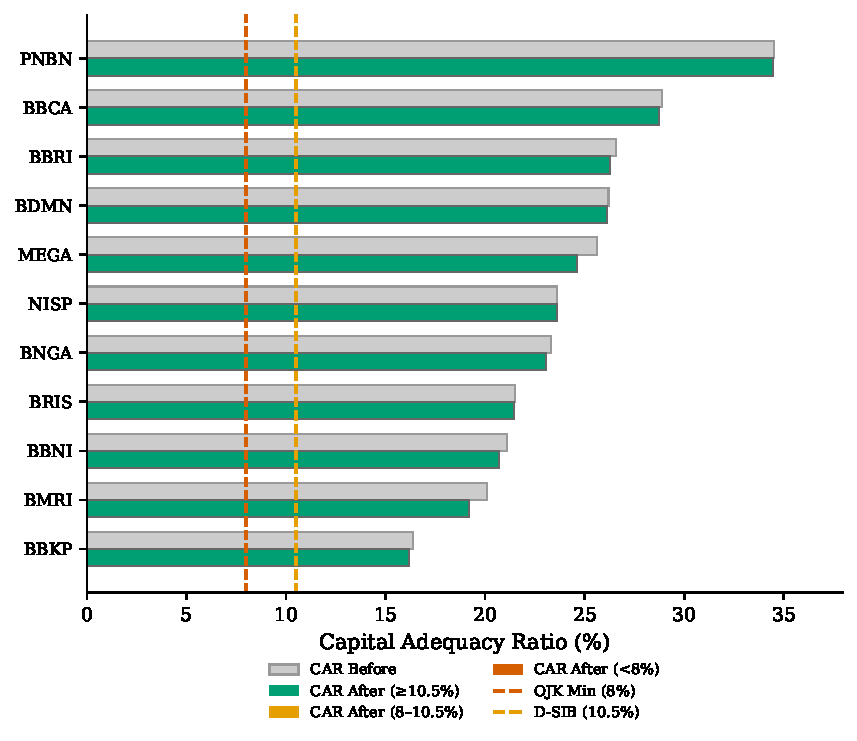
\includegraphics[width=\textwidth]{figures/fig_07.pdf}
\caption{Post-stress capital adequacy ratio (CAR) by bank under the 1.5\textdegree C scenario. Vertical dashed lines indicate the OJK minimum (8\%, red) and D-SIB buffer (10.5\%, orange). Banks are ordered by post-stress CAR.}
\label{fig:car_impact}
\end{figure}

\subsubsection{Aggregate Losses}

Under the 2\textdegree C scenario, total bank credit losses amount to \$1.8 billion, comprising \$1.6 billion in direct losses and \$254 million in indirect losses. This represents 2.12\% of system-wide bank equity. Under the 1.5\textdegree C scenario, total losses rise to \$3.1 billion (\$2.4 billion direct, \$762 million indirect), representing 3.60\% of system equity. While these aggregate losses are manageable at the system level, their distribution across banks is highly uneven.

\subsubsection{Bank-Level Vulnerability}

The concentration of coal exposure in a small number of large banks means that the stress test identifies specific institutions facing material losses. Bank Mandiri (BMRI) bears the largest absolute loss at \$1.6 billion under the 1.5\textdegree C scenario, driven by its dominant position in coal lending (\$1.2 billion in identified exposure plus substantial indirect mining loans). This loss represents 42.4\% of BMRI's pre-stress net income, indicating that over five months of earnings would be consumed by coal-related credit losses.

BMRI's post-stress CAR declines from 20.10\% to 19.21\% under the 1.5\textdegree C scenario, a 0.89 percentage point reduction, the largest CAR impact of any bank in our sample. This post-stress CAR remains well above both the OJK minimum of 8\% and the D-SIB buffer of 10.5\%, reflecting the substantial capital cushion that Indonesian D-SIBs have accumulated. No bank in our sample breaches either the OJK minimum or the D-SIB buffer under any scenario. Nevertheless, the concentration of losses (BMRI absorbs over 52\% of total system losses under 1.5\textdegree C) underscores the idiosyncratic vulnerability created by concentrated coal lending.

\subsubsection{Role of Existing Loan Loss Allowances (CKPN)}

Indonesian banks maintain loan loss allowances (Cadangan Kerugian Penurunan Nilai, or CKPN) as regulatory buffers against credit deterioration. These pre-existing provisions can absorb a portion of coal-related losses before they deplete equity capital. To assess this mitigating factor, we compute net losses after CKPN absorption: $L_b^{net,s} = \max(0, L_b^s - CKPN_b)$, where $CKPN_b$ is the bank's existing loan loss allowance. For banks without reported CKPN data, we apply the industry-average CKPN-to-loans ratio as a proxy.

When the CKPN buffer is incorporated, aggregate net losses decline, though the reduction varies across banks depending on their pre-existing provisioning levels. The CKPN-adjusted results indicate that major Indonesian banks have built sufficient provisioning buffers to absorb a meaningful share of the estimated coal-related credit losses. However, since existing CKPN is allocated across the entire loan portfolio (not exclusively for coal exposures), its availability for coal loss absorption may be more limited than the gross figures suggest. Our baseline results without the CKPN adjustment therefore represent a conservative upper bound on capital impact.

\subsubsection{Network Concentration}

Figure~\ref{fig:heatmap} presents a vulnerability heatmap for the 15 most exposed banks, combining information on coal exposure intensity, capital buffer adequacy, asset quality (NPL ratio), and profit absorption capacity. The heatmap reveals that vulnerability is not solely a function of exposure size: several mid-tier banks with smaller absolute exposures but thinner capital buffers and lower profitability face proportionally larger impacts.

\begin{figure}[htbp]
\centering
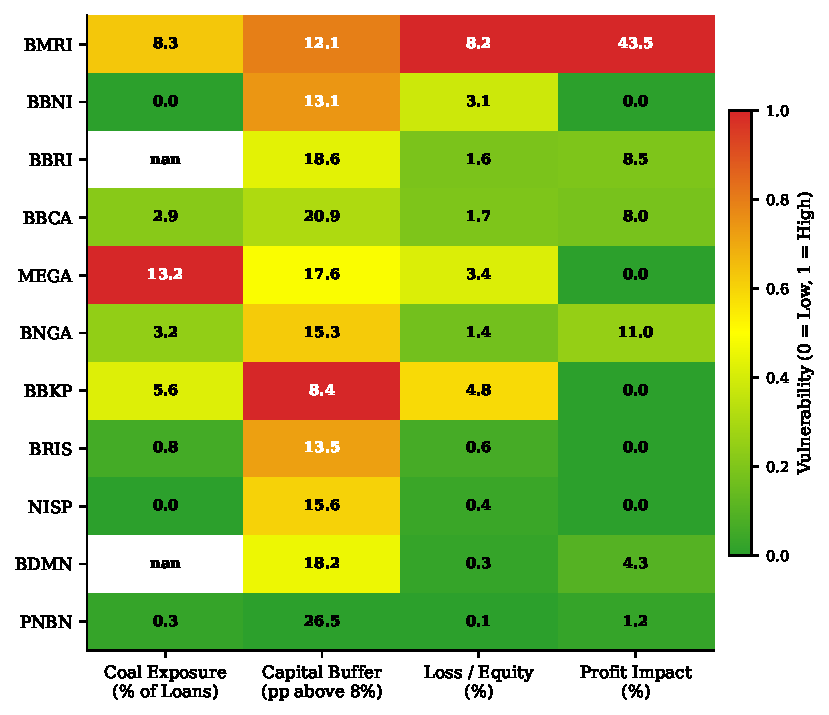
\includegraphics[width=\textwidth]{figures/fig_08.pdf}
\caption{Bank vulnerability heatmap. Rows represent the 15 most exposed banks; columns show normalised indicators of coal exposure intensity, capital buffer, NPL ratio, and profit impact. Darker shading indicates higher vulnerability. Values in cells show the original (un-normalised) metric.}
\label{fig:heatmap}
\end{figure}

The bipartite network structure (Figure~\ref{fig:network}) also reveals important features for systemic risk. The high degree of overlap, where multiple banks lend to the same coal companies and large coal companies borrow from multiple banks, creates potential for correlated losses. Under the 1.5\textdegree C scenario, 5 coal companies default and 10 are distressed simultaneously (among those with NPV data), meaning that banks cannot diversify away the coal stranding shock through portfolio breadth within the sector. This correlated default structure is consistent with the theoretical predictions of \citet{Acemoglu2015} regarding concentrated network topologies that amplify rather than absorb shocks.
